\chapter{Análisis del Problema}
    \section{QSS Bolivia}
        QSS Bolivia es una empresa boliviana dedicada a la asesoría, implementación y equipamiento de sistemas electrónicos de seguridad y automatización, que utiliza lo último de la tecnología para proteger y resguardar los bienes y asegurar la tranquilidad de sus clientes \parencite{QSSBolvia2016-el}
        \subsection{Situación Actual}
            QSS Bolivia se encuentra netamente conformada por profesionales bolivianos, formados principalmente en el área de informática y sistemas. La empresa cuenta con más de 10 años de trabajo, inicialmente enfocados principalmente al área de Consultoría Informática. Posteriormente, QSS Bolivia ingresó al área de seguridad de domicilios y empresas mediante la comercialización de dispositivos electrónicos orientados a la seguridad.
            Actualmente, las soluciones que proporciona QSS Bolivia en el área de vigilancia son implementadas mediante CCTV.
            
            El objetivo principal de la empresa es de otorgar soluciones alcanzando una sinergia cliente-proveedor, haciendo énfasis en las necesidades y requerimientos del proceso de seguridad que prevé el cliente.  
            Es esencial para QSS Bolivia invertir en capacitación del personal a fin de mantenerlo actualizado con los cambios tecnológicos que se presentan día a día y aprovechando al máximo las herramientas tecnológicas disponibles. 
            
            Finalmente, para QSS es importante el apoyo a la creación de Start-Ups asociados a nuevos emprendimientos de jóvenes estudiantes, tanto en el área de la informática y de la electrónica.
    \section{Análisis Preliminar de Requerimientos}
    \section{Escenario del Problema}
        \begin{figure}[H]
            \centering
            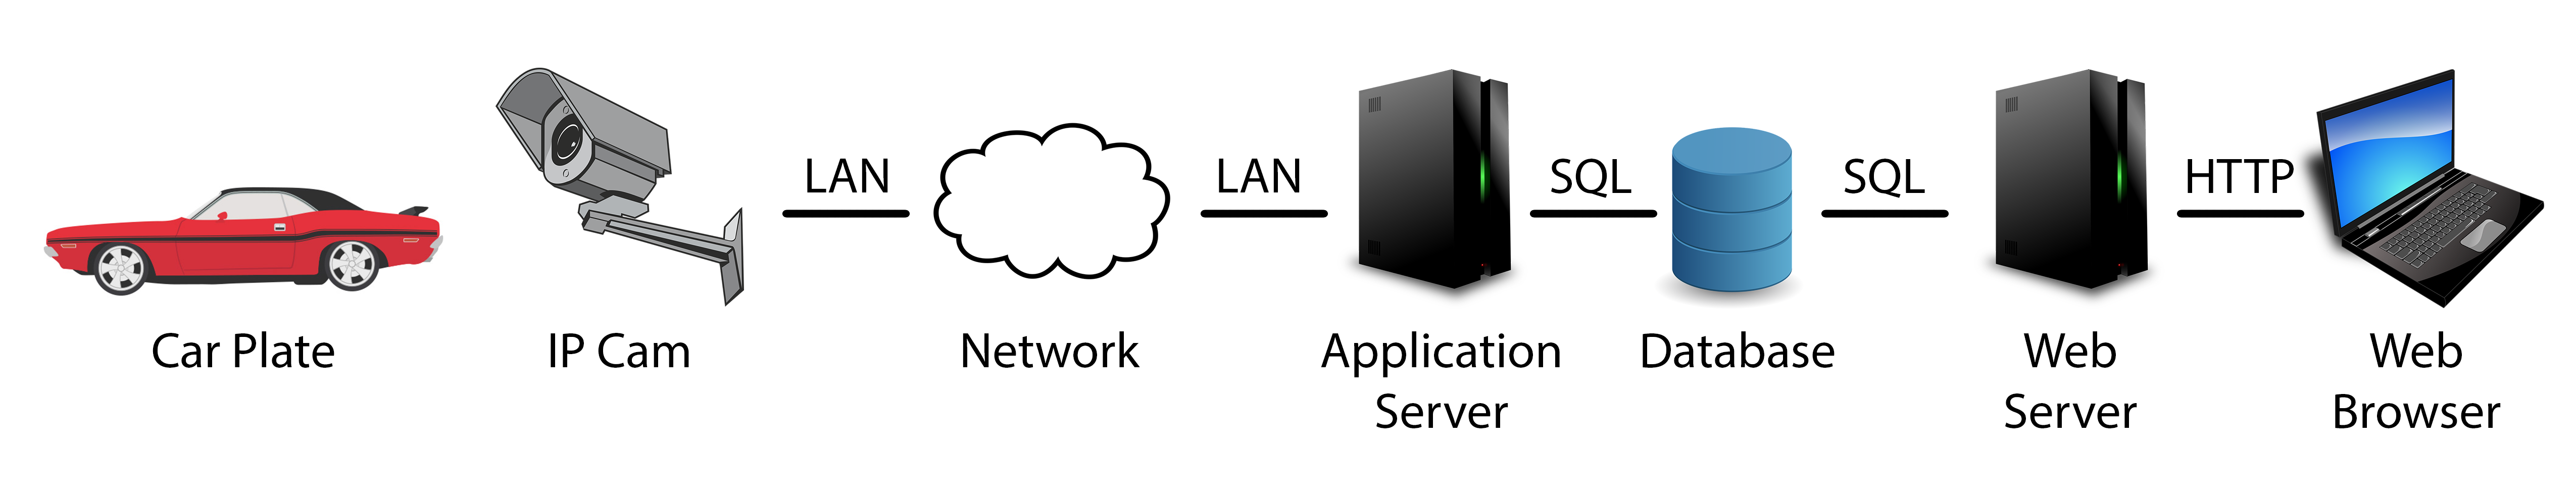
\includegraphics[width=0.90\textwidth]{nodos-overview}
            \caption{Panorama de los Nodos de la Aplicación}
            \label{fig:nodos-overview}
        \end{figure}
    
    Como se observa en la Figura \ref{fig:nodos-overview}, la aplicación distribuirá el nodo de aplicación, donde se ejecutaran los servicios Recolector y Reconocimiento; la base de datos; y, el servidor web, a través del cual el usuario accede a la información relacionada a los registros y al sistema.
        
        El proceso de reconocimiento de un vehículo sigue una cadena de procesos:

        \begin{enumerate}
            \item existe una cámara instalada y la información de la misma se encuentra almacenada en la base de datos
            \item el Servicio de Recolección de vídeo, una vez iniciado, reenvía el flujo de vídeo (cuadros) a un LB
            \item el LB distribuye los cuadros de vídeo recibidos entre los servicios de Reconocimiento disponibles
            \item el Servicio de Reconocimiento, por cada cuadro, ejecuta el algoritmo de reconocimiento y guarda en la BD si se reconoció una matricula
        \end{enumerate}    
        
        Toda la información de las matriculas reconocidas puede verse desde el cliente web.
        
        Bajo ese esquema, los servicios que componen a la aplicación pueden ser categorizados según su atomicidad:
        \begin{itemize}
            \item Servicios Atómicos: IaaS, Base de Datos, LB
            \item Servicios Compuestos: Servicio Recolector, Servicio de Reconocimiento, Servicio Web
        \end{itemize}
        De igual manera, pueden ser categorizados según su rol en la aplicación:
        \begin{itemize}
            \item Servicios Clave: Servicio Recolector, Servicio de Reconocimiento, LB, Servicio Web
            \item Servicios de Soporte: Base de Datos,
        \end{itemize}
    
        \begin{figure}[H]
            \centering
            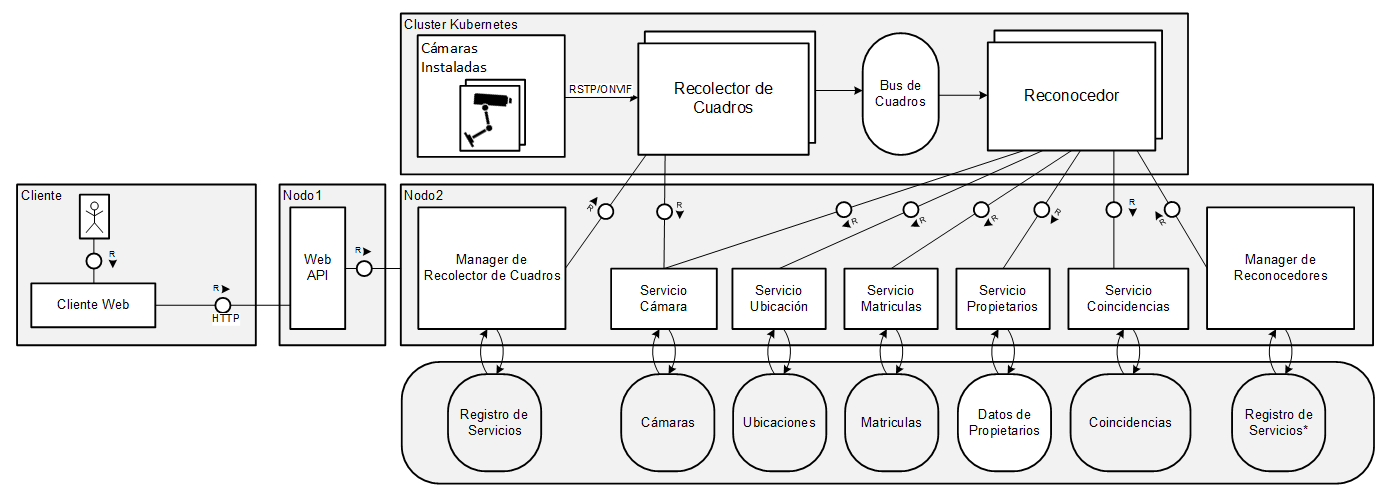
\includegraphics[width=1\textwidth]{nodos-arch}
            \caption{Arquitectura de la Aplicación}
            \label{fig:nodos-arch}
        \end{figure} 
        
        Dado el nivel de las tecnologías descrito en los capítulos 2-5, el proyecto utilizara:
        \begin{itemize}
            \item Kubernetes para la gestión y configuración de contendedores, dados los casos de uso exitosos en producción en compañías como Google, SAP, Ebay, Box \parencite{Kubernetes2016-ub}; y el poder de ser ejecutado en cualquier nube.
            \item OpenALPR sera utilizado para realizar el reconocimiento de matriculas, ya que utiliza OpenCV que es la tecnología principal en computación visual, además de ser open source, multiplataforma y ser utilizada por compañías como Microsoft, IBM, Intel, etc. \parencite{Itseez2000-he}.
            \item Se utilizara el Framework de desarrollo web Laravel, elegido en base a la experiencia del equipo de programadores con esta herramienta, la documentación que provee Laravel y las capacidades que posee, descritas en el Capitulo 5.
            \item Las cámaras que utiliza QSS Bolivia son de la marca Dahua. Las especificaciones se describen en el \todonum{Apendice} Apéndice X
        \end{itemize}

